\chapter{THỰC NGHIỆM}

\section{Quy Trình Thực Nghiệm}

\subsection{Xử Lý Dữ Liệu}

Quy trình chuẩn bị dữ liệu thực hiện qua hai notebook tuần tự:
\begin{itemize}
  \item \textbf{\texttt{00\_download\_datasets.ipynb}:} Tải bốn bộ Kaggle về \texttt{data/raw/}. Idempotent --- bỏ qua các bộ đã tồn tại.
  \item \textbf{\texttt{01\_dataset\_preparation.ipynb}:} MD5 dedup $\to$ class balance check $\to$ EDA plots $\to$ stratified split 70/15/15 $\to$ xuất CSV.
\end{itemize}

Kết quả: \textbf{316.530 ảnh} (221.571 train / 47.479 val / 47.480 test), phân bố nhãn đồng đều 47,3\% thật --- 52,7\% giả trên cả ba tập.

\subsection{Chuẩn Bị Dữ Liệu Cho Mô Hình}

\begin{itemize}
  \item \textbf{Tập train:} resize $224{\times}224$ $\to$ augmentation $\to$ chuẩn hóa ImageNet $\to$ \texttt{torch.Tensor}.
  \item \textbf{Tập val/test:} resize $224{\times}224$ $\to$ chuẩn hóa ImageNet (không augmentation).
  \item \textbf{DataLoader:} batch\_size=128, num\_workers=2, pin\_memory=True.
\end{itemize}

Seed tái lập cố định ở mức 42. Phiên bản ghi nhận khi bắt đầu chạy: PyTorch 2.12.0+cu130, timm 1.0.27, GPU NVIDIA GeForce RTX 5070.

\section{Độ Đo Đánh Giá}

Kết quả cuối cùng được báo cáo chỉ trên tập kiểm tra (47.480 ảnh), tính bằng \texttt{sklearn.metrics}.

\begin{table}[H]
  \centering
  \caption{Định nghĩa và ý nghĩa các độ đo đánh giá}
  \label{tab:metrics_def}
  \begin{tabularx}{\linewidth}{llX}
    \toprule
    \textbf{Độ đo} & \textbf{Công thức} & \textbf{Ý nghĩa trong bài toán} \\
    \midrule
    Accuracy  & $\frac{TP+TN}{TP+TN+FP+FN}$ & Tỷ lệ ảnh phân loại đúng tổng thể \\
    Precision & $\frac{TP}{TP+FP}$ & Trong số ảnh dự đoán là giả, bao nhiêu thực sự là giả \\
    Recall    & $\frac{TP}{TP+FN}$ & Trong số ảnh giả thực tế, bao nhiêu được phát hiện đúng \\
    F1-Score  & $\frac{2 \cdot P \cdot R}{P + R}$ & Trung bình điều hòa Precision và Recall \\
    AUC-ROC   & Diện tích dưới ROC & Khả năng phân biệt Real/Fake ở mọi ngưỡng threshold \\
    \bottomrule
  \end{tabularx}
\end{table}

Recall quan trọng hơn Precision vì bỏ sót ảnh giả (False Negative) gây hại thực tế nhiều hơn cảnh báo nhầm. AUC-ROC là độ đo tổng hợp tin cậy nhất vì không phụ thuộc vào ngưỡng phân loại cụ thể. \textit{Positive class} = Fake (1).

\section{Thông Số Chi Tiết Các Giai Đoạn Huấn Luyện}

\begin{table}[H]
  \centering
  \caption{Siêu tham số chung cho toàn bộ quá trình huấn luyện}
  \label{tab:hyperparam}
  \begin{tabular}{lll}
    \toprule
    \textbf{Tham số} & \textbf{Giá trị} & \textbf{Nguồn} \\
    \midrule
    Optimizer          & AdamW \cite{loshchilov2019adamw} & \texttt{train\_config.yaml} \\
    Weight decay       & $10^{-4}$                        & \texttt{train\_config.yaml} \\
    Batch size         & 128                              & \texttt{train\_config.yaml} \\
    Max epochs/stage   & 30                               & \texttt{train\_config.yaml} \\
    Mixed precision    & FP16 (autocast + GradScaler)     & \texttt{train\_config.yaml} \\
    EarlyStopping      & patience=5, monitor: val\_loss   & \texttt{train\_config.yaml} \\
    ReduceLROnPlateau  & patience=3, factor=0,3, min\_lr=$10^{-7}$ & \texttt{train\_config.yaml} \\
    Random seed        & 42                               & \texttt{train\_config.yaml} \\
    \bottomrule
  \end{tabular}
\end{table}

\section{Đánh Giá Thực Nghiệm}

\subsection{Kết Quả Trên Tập Kiểm Tra}

Đánh giá thực hiện trên tập kiểm tra độc lập (47.480 ảnh) với checkpoint tốt nhất của Giai đoạn 3 (\texttt{best\_stage3.pth}, val\_loss=$0{,}0699$).

\begin{table}[H]
  \centering
  \caption{Kết quả đánh giá trên tập kiểm tra --- checkpoint Stage 3}
  \label{tab:test_results}
  \begin{tabular}{lrr}
    \toprule
    \textbf{Độ đo} & \textbf{Giá trị} & \textbf{(\%)} \\
    \midrule
    Accuracy  & 0,9733 & 97,33\% \\
    Precision & 0,9773 & 97,73\% \\
    Recall    & 0,9718 & 97,18\% \\
    F1-Score  & 0,9745 & 97,45\% \\
    AUC-ROC   & 0,9970 & 99,70\% \\
    \bottomrule
  \end{tabular}
  \newline
  {\small Nguồn: \texttt{artifacts/results/metrics.txt}}
\end{table}

\begin{table}[H]
  \centering
  \caption{So sánh kết quả qua các giai đoạn trên tập kiểm định}
  \label{tab:stage_compare}
  \begin{tabular}{lccc}
    \toprule
    \textbf{Giai đoạn} & \textbf{Val Accuracy} & \textbf{Cải thiện} \\
    \midrule
    1 (Head only)       & 86,63\% & --- \\
    2 (Partial unfreeze) & 94,54\% & $+7{,}91$ pp \\
    3 (Full fine-tune)  & 97,34\% & $+2{,}80$ pp \\
    \bottomrule
  \end{tabular}
\end{table}

\begin{figure}[H]
  \centering
  \begin{subfigure}{0.48\linewidth}
    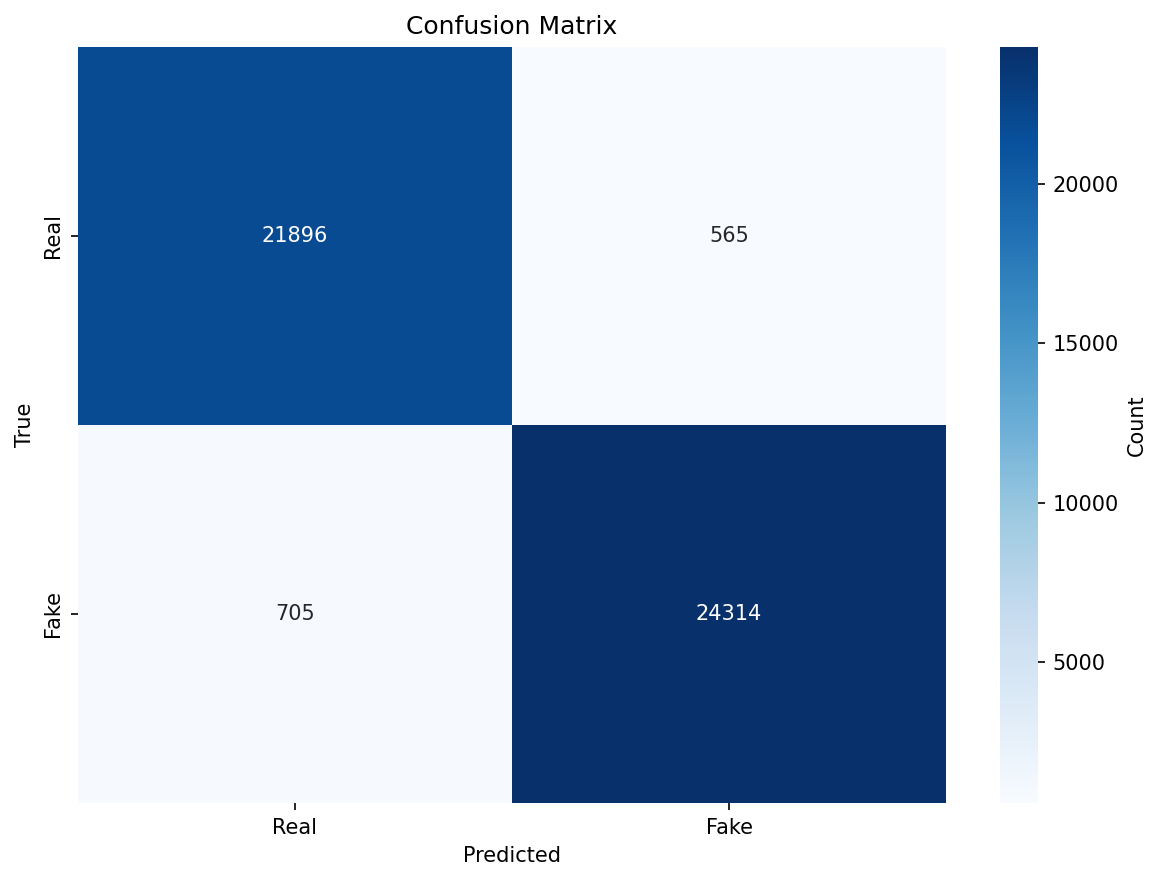
\includegraphics[width=\linewidth]{../../artifacts/results/confusion_matrix.png}
    \caption{Ma trận nhầm lẫn (tập test)}
    \label{fig:confusion}
  \end{subfigure}
  \hfill
  \begin{subfigure}{0.48\linewidth}
    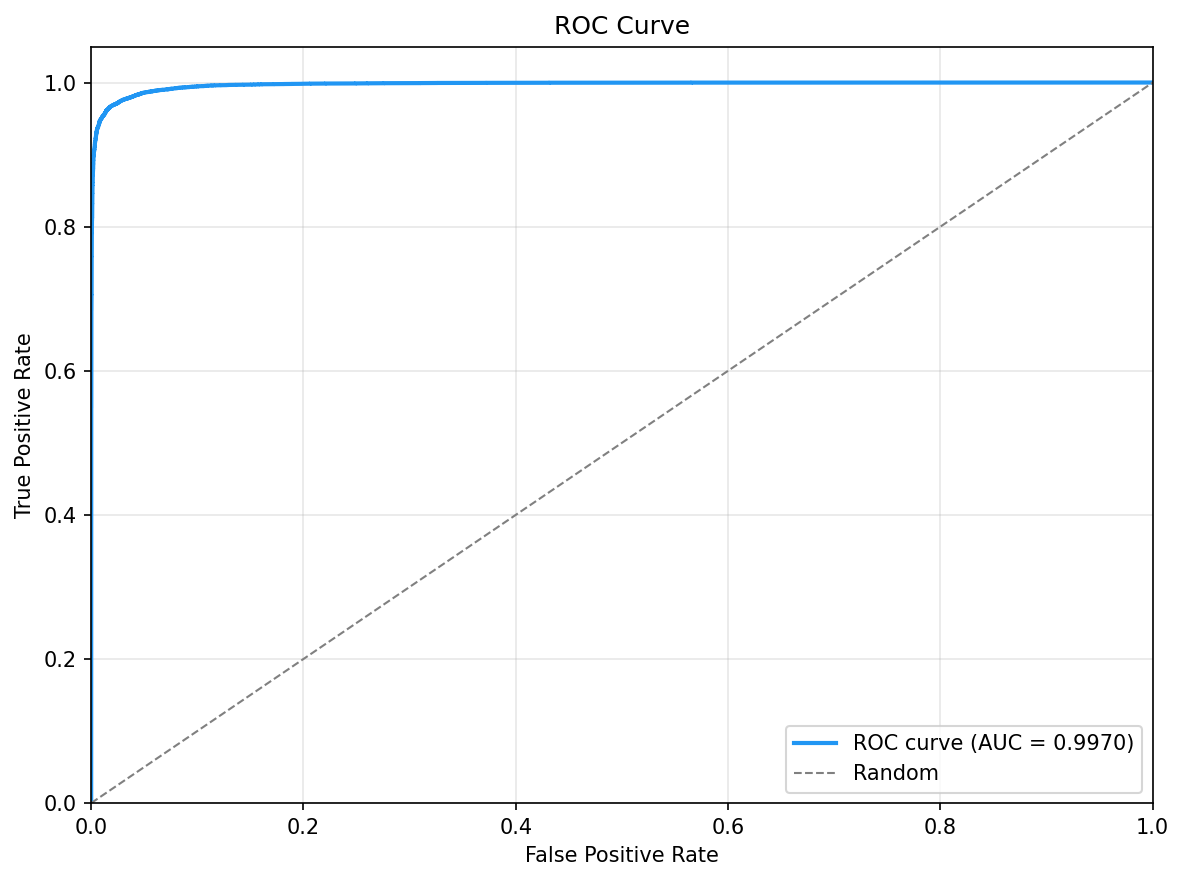
\includegraphics[width=\linewidth]{../../artifacts/results/roc_curve.png}
    \caption{Đường cong ROC (AUC = 0,9970)}
    \label{fig:roc}
  \end{subfigure}
  \caption{Kết quả đánh giá trên tập kiểm tra}
  \label{fig:eval_results}
\end{figure}

\begin{figure}[H]
  \centering
  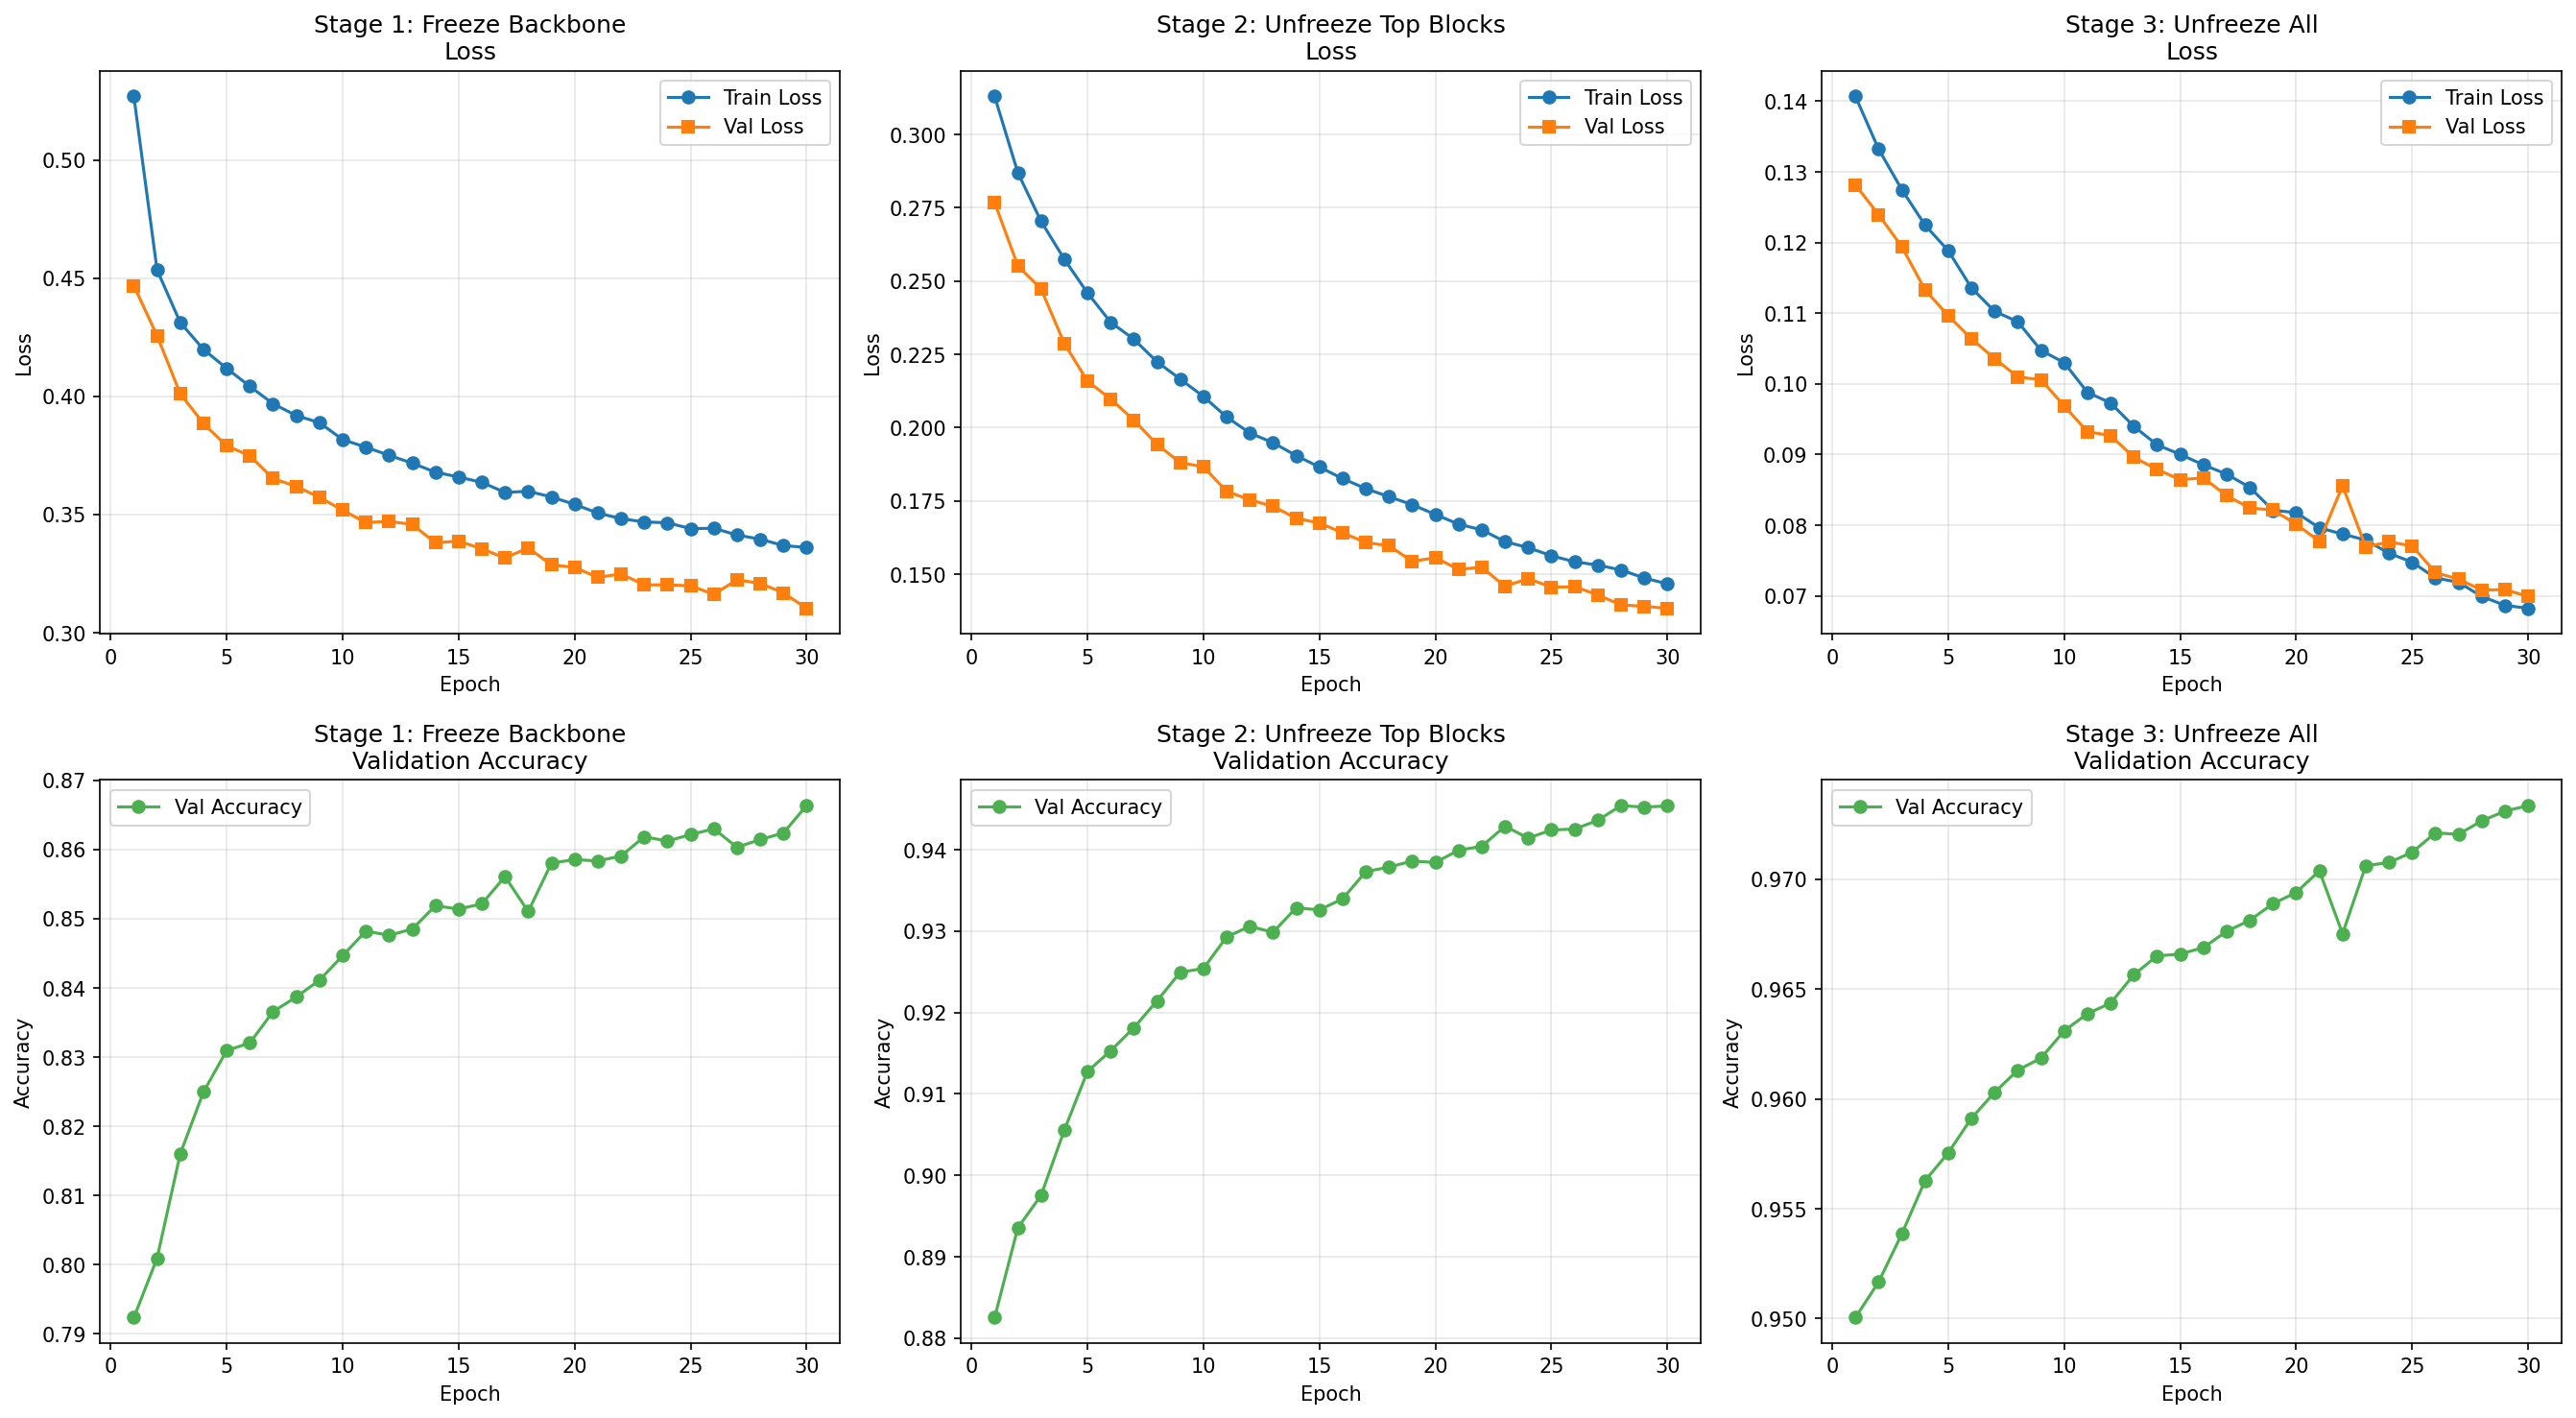
\includegraphics[width=0.9\linewidth]{../../artifacts/results/training_curves.png}
  \caption{Đường cong val\_loss và val\_accuracy theo epoch của 3 giai đoạn huấn luyện}
  \label{fig:training_curves}
\end{figure}

\subsection{Đánh Giá Cross-Generator}

Bài kiểm tra cross-generator thực hiện theo quy trình hold-out: lần lượt giữ lại từng bộ dữ liệu làm tập kiểm tra, huấn luyện mô hình trên ba bộ còn lại, sau đó đánh giá trên bộ bị giữ lại. Quy trình này được lặp lại bốn lần --- một lần cho mỗi bộ dữ liệu. Hình~\ref{fig:cross_gen_scheme} minh họa sơ đồ tổng quát của quy trình này.

\begin{figure}[H]
  \centering
  \begin{tikzpicture}[
    every node/.style={font=\footnotesize},
    trn/.style   = {rectangle, draw=uitblue, fill=uitblue!10, rounded corners=3pt,
                    minimum width=5.0cm, minimum height=0.75cm, align=center},
    hld/.style   = {rectangle, draw=red!60, fill=red!8, rounded corners=3pt,
                    minimum width=1.9cm, minimum height=0.75cm, align=center},
    res/.style   = {rectangle, draw=green!60!black, fill=green!7, rounded corners=3pt,
                    minimum width=2.2cm, minimum height=0.75cm, align=center},
    arr/.style   = {-Stealth, semithick}
  ]
    % Column headers
    \node[font=\footnotesize\bfseries] at (-1.2,  0.55) {Holdout};
    \node[font=\footnotesize\bfseries] at ( 3.1,  0.55) {Huấn luyện (3 bộ)};
    \node[font=\footnotesize\bfseries] at ( 7.0,  0.55) {Accuracy};
    \node[font=\footnotesize\bfseries] at ( 9.4,  0.55) {AUC-ROC};

    % Row 1
    \node[hld] (h1) at (-1.2,  0)    {StyleGAN};
    \node[trn] (t1) at ( 3.1,  0)    {Deepfake + HardFake + ciplab};
    \node[res] (a1) at ( 7.0,  0)    {99,04\%};
    \node[res] (u1) at ( 9.4,  0)    {99,95\%};
    \draw[arr] (t1.east) -- (a1.west);

    % Row 2
    \node[hld] (h2) at (-1.2, -1.15) {Deepfake};
    \node[trn] (t2) at ( 3.1, -1.15) {StyleGAN + HardFake + ciplab};
    \node[res] (a2) at ( 7.0, -1.15) {96,50\%};
    \node[res] (u2) at ( 9.4, -1.15) {99,55\%};
    \draw[arr] (t2.east) -- (a2.west);

    % Row 3
    \node[hld] (h3) at (-1.2, -2.3)  {HardFake};
    \node[trn] (t3) at ( 3.1, -2.3)  {StyleGAN + Deepfake + ciplab};
    \node[res] (a3) at ( 7.0, -2.3)  {90,77\%};
    \node[res] (u3) at ( 9.4, -2.3)  {97,07\%};
    \draw[arr] (t3.east) -- (a3.west);

    % Row 4 (ciplab — red highlight)
    \node[hld, fill=red!15] (h4) at (-1.2, -3.45) {ciplab};
    \node[trn]              (t4) at ( 3.1, -3.45) {StyleGAN + Deepfake + HardFake};
    \node[res, fill=red!15] (a4) at ( 7.0, -3.45) {53,36\%};
    \node[res, fill=red!15] (u4) at ( 9.4, -3.45) {53,44\%};
    \draw[arr] (t4.east) -- (a4.west);
  \end{tikzpicture}
  \caption{Sơ đồ quy trình đánh giá cross-generator (hold-out từng bộ dữ liệu).
           Ô đỏ đậm: bộ ciplab gây sụp đổ hoàn toàn khi bị giữ lại.}
  \label{fig:cross_gen_scheme}
\end{figure}

\begin{table}[H]
  \centering
  \caption{Kết quả cross-generator evaluation đầy đủ (5 độ đo)}
  \label{tab:cross_gen}
  \begin{tabular}{lrrrrr}
    \toprule
    \textbf{Holdout} & \textbf{Acc} & \textbf{Prec} & \textbf{Recall} & \textbf{F1} & \textbf{AUC} \\
    \midrule
    140k-StyleGAN & 99,04\% & 98,93\% & 99,13\% & 99,03\% & 99,95\% \\
    Deepfake-Real & 96,50\% & 97,11\% & 96,55\% & 96,83\% & 99,55\% \\
    Hard-FakeReal & 90,77\% & 88,46\% & 93,88\% & 91,09\% & 97,07\% \\
    ciplab        & 53,36\% & 50,88\% & 20,71\% & 29,44\% & 53,44\% \\
    \bottomrule
  \end{tabular}
  \newline
  {\small Nguồn: \texttt{reports/cross\_generator/cross\_generator\_metrics.json}}
\end{table}

\subsection{Đánh Giá Robustness}

\begin{table}[H]
  \centering
  \caption{Kết quả robustness evaluation}
  \label{tab:robustness}
  \begin{tabular}{lrrr}
    \toprule
    \textbf{Điều kiện nhiễu} & \textbf{Accuracy} & \textbf{F1-Score} & \textbf{AUC-ROC} \\
    \midrule
    Baseline (không nhiễu) & 0,9733 & 0,9745 & 0,9970 \\
    JPEG nén $q=70$        & 82,33\% & 85,32\% & 95,97\% \\
    JPEG nén $q=50$        & 79,77\% & 83,45\% & 93,30\% \\
    JPEG nén $q=30$        & 78,60\% & 82,48\% & 90,30\% \\
    Downscale 50\%         & 85,39\% & 85,60\% & 93,58\% \\
    Downscale 25\%         & 72,87\% & 75,85\% & 80,40\% \\
    Gaussian blur $\sigma=1$ & 90,45\% & 90,29\% & 97,76\% \\
    Gaussian blur $\sigma=2$ & 73,65\% & 73,84\% & 82,11\% \\
    \bottomrule
  \end{tabular}
  \newline
  {\small Nguồn: \texttt{reports/robustness/robustness\_metrics.json}}
\end{table}

\subsection{Nhận Xét}

\subsubsection{Đánh Giá Tổng Quan}

Mô hình EfficientNet-B0 sau Giai đoạn 3 đạt kết quả xuất sắc trên tập kiểm tra chuẩn với Accuracy 97,33\%, F1-Score 97,45\% và AUC-ROC 99,70\%. Val accuracy cải thiện tổng cộng $+10{,}71$ điểm phần trăm từ Giai đoạn 1 đến Giai đoạn 3, xác nhận hiệu quả của chiến lược progressive unfreezing.

\subsubsection{Đánh Giá Theo Từng Độ Đo}

\textbf{Precision (0,9773):} Khi mô hình dự đoán một ảnh là giả, xác suất đúng đạt 97,73\%. Precision cao bác bỏ giả thuyết mô hình thiên vị về lớp đa số (53\% Fake).

\textbf{Recall (0,9718):} Mô hình phát hiện được 97,18\% tổng số ảnh giả thực tế. Khoảng cách nhỏ giữa Precision và Recall ($0{,}55$ pp) cho thấy mô hình không thiên lệch đáng kể về phía nào.

\textbf{AUC-ROC (0,9970):} Gần hoàn hảo --- mô hình có khả năng phân tách xác suất thật/giả rất tốt ở mọi mức ngưỡng.

\subsubsection{Phân Tích Nguyên Nhân Thành Công}

\begin{itemize}
  \item \textbf{Quy mô dữ liệu đa nguồn:} 316.530 ảnh từ 4 phương pháp sinh buộc mô hình học đặc trưng phổ quát thay vì phụ thuộc vào artifact của một phương pháp cụ thể.
  \item \textbf{Progressive unfreezing:} Ngăn catastrophic forgetting, cho phép backbone thích nghi dần với domain khuôn mặt.
  \item \textbf{Mixed precision FP16:} Cho phép batch size 128, cung cấp gradient estimate ổn định hơn.
  \item \textbf{EarlyStopping không kích hoạt:} Cho thấy 30 epochs là hợp lý --- mô hình chưa overfitting khi kết thúc; tăng thêm epochs có thể cải thiện thêm.
\end{itemize}

\subsubsection{Trực Quan Hóa Grad-CAM}

Grad-CAM được thực hiện trên 32 ảnh mẫu (4 Real + 4 Fake $\times$ 4 nguồn), sử dụng checkpoint Stage~3 với lớp mục tiêu là \texttt{backbone.blocks[-1]} (MBConv block cuối của EfficientNet-B0). Kết quả đạt 30/32 dự đoán đúng (93,8\%) trên tập mẫu này --- hai ảnh sai đều thuộc bộ ciplab, nhất quán với kết quả cross-generator (AUC 53,44\%).

\begin{figure}[H]
  \centering
  
\includegraphics[width=\linewidth]{../gradcam/gradcam_grid.png}
  \caption{Grid Grad-CAM overlay 32 ảnh mẫu (4 nguồn $\times$ 4 Real + 4 Fake). Tiêu đề xanh lá = dự đoán đúng, đỏ = sai.}
  \label{fig:gradcam_grid}
\end{figure}

Quan sát vùng kích hoạt theo nguồn cho thấy:
\begin{itemize}
  \item \textbf{140k-StyleGAN và Hard-FakeReal:} Activation tập trung rõ ràng vào vùng trung tâm khuôn mặt (mắt, sống mũi) và lan sang biên tóc--da --- nơi artifact GAN phổ biến nhất. Cả 8/8 mẫu đúng ở cả hai nguồn.
  \item \textbf{Deepfake-Real:} Activation phân bổ rộng hơn trên toàn khuôn mặt, đặc biệt ở vùng mắt và biên ghép khuôn mặt --- đúng với cơ chế artifact của manipulation-based deepfake. Đạt 8/8.
  \item \textbf{ciplab:} Heatmap kém tập trung, thường lan ra vùng nền hoặc cổ --- cho thấy mô hình không tìm được vùng artifact đặc trưng của nguồn này. Hai ảnh sai có activation phân tán toàn ảnh.
\end{itemize}

Kết quả xác nhận mô hình học chiến lược phát hiện dựa trên vùng khuôn mặt có ngữ nghĩa thay vì đặc trưng màu sắc toàn cục --- tín hiệu tích cực về tính tin cậy. Sự kém tập trung trên ciplab nhất quán với giới hạn cross-generator và chỉ ra rằng artifact ciplab GAN nằm ngoài không gian đặc trưng đã học.

\subsection{Phân Tích Lỗi}

Dựa trên ma trận nhầm lẫn, kết quả cross-generator, kết quả robustness và quan sát Grad-CAM, các trường hợp lỗi phân loại được phân thành ba nhóm chính:

\textbf{Nhóm 1 --- False Negative: ảnh giả bị phân loại là thật.}
Nhóm này chủ yếu gồm ảnh từ bộ ciplab khi holdout (Recall chỉ 20,71\%) và một phần từ Hard-FakeReal. Đặc điểm chung là không có artifact tần số cao rõ ràng --- Grad-CAM cho heatmap phân tán. Đây là trường hợp mô hình thiếu đặc trưng phân biệt thực sự, không thể cải thiện bằng hyperparameter tuning mà cần bổ sung dữ liệu từ chính generator đó.

\textbf{Nhóm 2 --- False Positive: ảnh thật bị phân loại là giả.}
Nhóm này tăng mạnh khi ảnh bị nén JPEG. Tại $q=70$, Precision giảm từ 97,73\% xuống 75,88\%, tức là gần 1/4 ảnh bị cảnh báo nhầm là giả. Nguyên nhân: nén JPEG tạo ra blocking artifact ở tần số trung-cao tương tự artifact GAN, làm mô hình nhầm. Đây là lỗi hệ thống có thể giảm bằng cách thêm \texttt{ImageCompression} vào pipeline augmentation.

\textbf{Nhóm 3 --- Lỗi do mất thông tin nặng.}
Khi downscale $\times 0{,}25$ hoặc Gaussian blur $\sigma=2$, cả False Negative lẫn False Positive đều tăng vì thông tin tần số cao --- nguồn đặc trưng chính của mô hình --- bị xóa vĩnh viễn. Không có biện pháp tiền xử lý nào có thể phục hồi thông tin đã mất; chỉ có super-resolution trước khi phân loại có thể giảm nhẹ tác động.

\begin{table}[H]
  \centering
  \caption{Tóm tắt phân tích lỗi theo điều kiện}
  \label{tab:error_analysis}
  \begin{tabularx}{\linewidth}{lXl}
    \toprule
    \textbf{Điều kiện} & \textbf{Loại lỗi chủ đạo} & \textbf{Biện pháp đề xuất} \\
    \midrule
    ciplab holdout    & FN cao (Recall 20,71\%) & Bổ sung ảnh ciplab vào train \\
    Hard-FakeReal holdout & FN tăng (Acc 90,77\%) & Tăng augmentation độ khó \\
    JPEG $q \leq 70$  & FP tăng (Prec giảm $\approx$22 pp) & Thêm \texttt{ImageCompression} augmentation \\
    Downscale $\times 0{,}25$ & Cả FN và FP tăng & Thêm downscale augmentation \\
    Blur $\sigma=2$   & Cả FN và FP tăng & Thêm Gaussian blur augmentation \\
    \bottomrule
  \end{tabularx}
\end{table}

\section{Ứng Dụng Thực Nghiệm}

\subsection{Pipeline Inference}

\subsection{Sơ Đồ Pipeline Inference}

Hình~\ref{fig:inference_pipeline} trực quan hóa từng bước trong quy trình phân loại một ảnh mới, từ file đầu vào đến quyết định Real/Fake cuối cùng.

\begin{figure}[H]
  \centering
  \begin{tikzpicture}[
    node distance=0.52cm,
    every node/.style={font=\small},
    proc/.style = {rectangle, draw=uitblue, fill=uitblue!8, rounded corners=3pt,
                   minimum width=9.5cm, minimum height=0.88cm, align=center},
    dec/.style  = {diamond, draw=orange!70!black, fill=orange!8, aspect=3,
                   minimum height=1.1cm, align=center},
    res/.style  = {rectangle, draw=green!60!black, fill=green!7, rounded corners=3pt,
                   minimum width=3.5cm, minimum height=0.8cm, align=center},
    arr/.style  = {-Stealth, semithick}
  ]
    \node[proc] (i1) {Ảnh đầu vào (định dạng bất kỳ)};
    \node[proc, below=of i1] (i2) {\texttt{PIL.Image.open()} $\to$ \texttt{convert("RGB")}};
    \node[proc, below=of i2] (i3) {Resize($224\times224$) $\to$ Normalize(ImageNet) $\to$ \texttt{ToTensorV2}};
    \node[proc, below=of i3] (i4) {\texttt{unsqueeze(0)} --- Thêm batch dimension};
    \node[proc, below=of i4] (i5) {\texttt{model.eval()} \quad Forward pass};
    \node[proc, below=of i5] (i6) {\texttt{torch.sigmoid(logit)} $\to$ xác suất $p \in [0,1]$};
    \node[dec,  below=0.65cm of i6] (dec) {$p > 0{,}5$?};
    \node[res, below left=0.65cm and 1.6cm of dec]  (fake) {\textbf{Fake}\\(Ảnh giả mạo)};
    \node[res, below right=0.65cm and 1.6cm of dec] (real) {\textbf{Real}\\(Ảnh thật)};

    \foreach \a/\b in {i1/i2, i2/i3, i3/i4, i4/i5, i5/i6, i6/dec}
      \draw[arr] (\a.south) -- (\b.north);

    \draw[arr] (dec.south west)
      -- node[left, font=\footnotesize] {Có} (fake.north);
    \draw[arr] (dec.south east)
      -- node[right, font=\footnotesize] {Không} (real.north);
  \end{tikzpicture}
  \caption{Pipeline inference phân loại ảnh mới (ngưỡng mặc định 0,5)}
  \label{fig:inference_pipeline}
\end{figure}

\begin{lstlisting}[style=python, caption={Pipeline phân loại ảnh mới}]
from PIL import Image
import torch, albumentations as A
from albumentations.pytorch import ToTensorV2

transform = A.Compose([
    A.Resize(224, 224),
    A.Normalize(mean=[0.485,0.456,0.406],
                std=[0.229,0.224,0.225]),
    ToTensorV2()
])

model.eval()
with torch.no_grad():
    img = transform(image=np.array(Image.open(path).convert("RGB")))
    logit = model(img["image"].unsqueeze(0).to(device))
    prob  = torch.sigmoid(logit).item()
    label = "Fake" if prob > 0.5 else "Real"
\end{lstlisting}

Ngưỡng mặc định là $0{,}5$. Trong ứng dụng ưu tiên Recall cao (không bỏ sót ảnh giả), ngưỡng có thể được hạ xuống $0{,}3$--$0{,}4$ dựa trên đường ROC.
